% Options for packages loaded elsewhere
\PassOptionsToPackage{unicode}{hyperref}
\PassOptionsToPackage{hyphens}{url}
\PassOptionsToPackage{dvipsnames,svgnames,x11names}{xcolor}
%
\documentclass[
  letterpaper,
  DIV=11,
  numbers=noendperiod]{scrartcl}

\usepackage{amsmath,amssymb}
\usepackage{iftex}
\ifPDFTeX
  \usepackage[T1]{fontenc}
  \usepackage[utf8]{inputenc}
  \usepackage{textcomp} % provide euro and other symbols
\else % if luatex or xetex
  \usepackage{unicode-math}
  \defaultfontfeatures{Scale=MatchLowercase}
  \defaultfontfeatures[\rmfamily]{Ligatures=TeX,Scale=1}
\fi
\usepackage{lmodern}
\ifPDFTeX\else  
    % xetex/luatex font selection
\fi
% Use upquote if available, for straight quotes in verbatim environments
\IfFileExists{upquote.sty}{\usepackage{upquote}}{}
\IfFileExists{microtype.sty}{% use microtype if available
  \usepackage[]{microtype}
  \UseMicrotypeSet[protrusion]{basicmath} % disable protrusion for tt fonts
}{}
\makeatletter
\@ifundefined{KOMAClassName}{% if non-KOMA class
  \IfFileExists{parskip.sty}{%
    \usepackage{parskip}
  }{% else
    \setlength{\parindent}{0pt}
    \setlength{\parskip}{6pt plus 2pt minus 1pt}}
}{% if KOMA class
  \KOMAoptions{parskip=half}}
\makeatother
\usepackage{xcolor}
\setlength{\emergencystretch}{3em} % prevent overfull lines
\setcounter{secnumdepth}{-\maxdimen} % remove section numbering
% Make \paragraph and \subparagraph free-standing
\makeatletter
\ifx\paragraph\undefined\else
  \let\oldparagraph\paragraph
  \renewcommand{\paragraph}{
    \@ifstar
      \xxxParagraphStar
      \xxxParagraphNoStar
  }
  \newcommand{\xxxParagraphStar}[1]{\oldparagraph*{#1}\mbox{}}
  \newcommand{\xxxParagraphNoStar}[1]{\oldparagraph{#1}\mbox{}}
\fi
\ifx\subparagraph\undefined\else
  \let\oldsubparagraph\subparagraph
  \renewcommand{\subparagraph}{
    \@ifstar
      \xxxSubParagraphStar
      \xxxSubParagraphNoStar
  }
  \newcommand{\xxxSubParagraphStar}[1]{\oldsubparagraph*{#1}\mbox{}}
  \newcommand{\xxxSubParagraphNoStar}[1]{\oldsubparagraph{#1}\mbox{}}
\fi
\makeatother


\providecommand{\tightlist}{%
  \setlength{\itemsep}{0pt}\setlength{\parskip}{0pt}}\usepackage{longtable,booktabs,array}
\usepackage{calc} % for calculating minipage widths
% Correct order of tables after \paragraph or \subparagraph
\usepackage{etoolbox}
\makeatletter
\patchcmd\longtable{\par}{\if@noskipsec\mbox{}\fi\par}{}{}
\makeatother
% Allow footnotes in longtable head/foot
\IfFileExists{footnotehyper.sty}{\usepackage{footnotehyper}}{\usepackage{footnote}}
\makesavenoteenv{longtable}
\usepackage{graphicx}
\makeatletter
\def\maxwidth{\ifdim\Gin@nat@width>\linewidth\linewidth\else\Gin@nat@width\fi}
\def\maxheight{\ifdim\Gin@nat@height>\textheight\textheight\else\Gin@nat@height\fi}
\makeatother
% Scale images if necessary, so that they will not overflow the page
% margins by default, and it is still possible to overwrite the defaults
% using explicit options in \includegraphics[width, height, ...]{}
\setkeys{Gin}{width=\maxwidth,height=\maxheight,keepaspectratio}
% Set default figure placement to htbp
\makeatletter
\def\fps@figure{htbp}
\makeatother

\KOMAoption{captions}{tableheading}
\makeatletter
\@ifpackageloaded{caption}{}{\usepackage{caption}}
\AtBeginDocument{%
\ifdefined\contentsname
  \renewcommand*\contentsname{Table of contents}
\else
  \newcommand\contentsname{Table of contents}
\fi
\ifdefined\listfigurename
  \renewcommand*\listfigurename{List of Figures}
\else
  \newcommand\listfigurename{List of Figures}
\fi
\ifdefined\listtablename
  \renewcommand*\listtablename{List of Tables}
\else
  \newcommand\listtablename{List of Tables}
\fi
\ifdefined\figurename
  \renewcommand*\figurename{Figure}
\else
  \newcommand\figurename{Figure}
\fi
\ifdefined\tablename
  \renewcommand*\tablename{Table}
\else
  \newcommand\tablename{Table}
\fi
}
\@ifpackageloaded{float}{}{\usepackage{float}}
\floatstyle{ruled}
\@ifundefined{c@chapter}{\newfloat{codelisting}{h}{lop}}{\newfloat{codelisting}{h}{lop}[chapter]}
\floatname{codelisting}{Listing}
\newcommand*\listoflistings{\listof{codelisting}{List of Listings}}
\makeatother
\makeatletter
\makeatother
\makeatletter
\@ifpackageloaded{caption}{}{\usepackage{caption}}
\@ifpackageloaded{subcaption}{}{\usepackage{subcaption}}
\makeatother
\ifLuaTeX
  \usepackage{selnolig}  % disable illegal ligatures
\fi
\usepackage{bookmark}

\IfFileExists{xurl.sty}{\usepackage{xurl}}{} % add URL line breaks if available
\urlstyle{same} % disable monospaced font for URLs
\hypersetup{
  pdftitle={Structural Estimation of Life Cycle Models with Wealth in the Utility Function},
  pdfauthor={Alan Lujan},
  colorlinks=true,
  linkcolor={blue},
  filecolor={Maroon},
  citecolor={Blue},
  urlcolor={Blue},
  pdfcreator={LaTeX via pandoc}}

\title{Structural Estimation of Life Cycle Models with Wealth in the
Utility Function}
\usepackage{etoolbox}
\makeatletter
\providecommand{\subtitle}[1]{% add subtitle to \maketitle
  \apptocmd{\@title}{\par {\large #1 \par}}{}{}
}
\makeatother
\subtitle{CEF 2024 NTU Singapore}
\author{Alan Lujan}
\date{2024-06-20}

\begin{document}
\maketitle

\subsection{Why do people save?}\label{why-do-people-save}

Reasons for Saving

Can't save

Education

Family

Home

Investment

Liquidity/the future

No particular reason

Purchases

Retirement

edcl\_lbl

Bachelors degree or higher

2.06\%

8.86\%

3.67\%

3.63\%

2.35\%

33.81\%

1.11\%

6.98\%

37.53\%

high school diploma or GED

5.22\%

7.98\%

5.75\%

4.79\%

2.64\%

35.04\%

1.09\%

11.87\%

25.62\%

no high school diploma/GED

10.54\%

7.35\%

6.73\%

4.42\%

3.01\%

33.67\%

1.26\%

15.04\%

17.99\%

some college or Assoc. degree

3.63\%

8.79\%

4.82\%

4.58\%

2.61\%

35.97\%

1.12\%

10.70\%

27.78\%

\subsection{Life Cycle savings
profiles}\label{life-cycle-savings-profiles}

Insert graphs from SCF normalized and unnormalized

\subsection{Motivation and Research
Quesitions}\label{motivation-and-research-quesitions}

\subsubsection{Motivation}\label{motivation}

\begin{itemize}
\tightlist
\item
  Wealth accumulation
\item
  Inequality
\item
  Life Cycle / Retirement
\end{itemize}

\subsubsection{Research Questions}\label{research-questions}

\begin{itemize}
\tightlist
\item
  What are these models missing?
\item
  How do we better fit the distribution of wealth at the top?
\item
  How much does wealth in the utility function matter?
\item
  How imporant are life cycle properties?
\end{itemize}

\[
\newcommand{\DiscFac}{\beta}
\newcommand{\cFunc}{\mathrm{c}}
\newcommand{\uFunc}{\mathrm{u}}
\newcommand{\vFunc}{\mathrm{v}}
\newcommand{\Alive}{\mathcal{L}}
\newcommand{\h}{h}
\newcommand{\cLvl}{\mathbf{c}}
\newcommand{\mLvl}{\mathbf{m}}
\newcommand{\pLvl}{\mathbf{p}}
\newcommand{\Ex}{\mathbb{E}}
\newcommand{\CRRA}{\rho}
\newcommand{\PermGroFac}{\pmb{\Phi}}
\newcommand{\Rfree}{\mathsf{R}}
\newcommand{\PermShk}{\mathbf{\Psi}}
\newcommand{\TranShk}{\pmb{\xi}}
\newcommand{\aNrm}{a}
\newcommand{\cNrm}{c}
\newcommand{\RNrm}{\mathcal{R}}
\newcommand{\TranShkEmp}{\pmb{\theta}}
\newcommand{\mNrm}{m}
\newcommand{\pZero}{\wp}
\newcommand{\aFunc}{\mathrm{a}}
\newcommand{\kapShare}{\alpha}
\newcommand{\wealth}{o}
\newcommand{\kap}{k}
\newcommand{\wealthShare}{\delta}
\newcommand{\wFunc}{\mathrm{w}}
\newcommand{\aRat}{a}
\newcommand{\mRat}{m}
\newcommand{\aMat}{[\mathrm{a}]}
\newcommand{\mMat}{[\mathrm{m}]}
\newcommand{\weight}{\omega}
\]

\subsection{Some Literature}\label{some-literature}

\begin{itemize}
\item
  Why do the rich save so much? - Carroll {[}1998{]}

  \begin{itemize}
  \tightlist
  \item
    the rich have higher lifetime savings rates
  \item
    models of consumption smoothing and precautionary savings can not
    explain this
  \item
    propose a model where wealth is in the utility function
  \item
    households derive utility from wealth itself OR
  \item
    wealth provides a flow of services such as political power or social
    status
  \end{itemize}
\item
  Do the rich save more? - Dyan Skinner Zeldes {[}2004{]}
\end{itemize}

\subsection{The baseline LCIM model}\label{the-baseline-lcim-model}

\paragraph{Life Cycle Incomplete Markets
Model}\label{life-cycle-incomplete-markets-model}

The agent maximizes PDV of utility from consumption over life cycle with
terminal period \(T\):

\[\begin{equation}
\label{eq:lifecyclemax}
\vFunc_{t}(\pLvl_{t},\mLvl_{t})  = \max_{\{\cFunc\}_{t}^{T}} ~ \uFunc(\cLvl_{t})+\Ex_{t}\left[\sum_{n=1}^{T-t} {\beth}^{n} \Alive_{t}^{t+n}\hat{\DiscFac}_{t}^{t+n} \uFunc(\cLvl_{t+n}) \right]
\end{equation}\]

where \(\pLvl_{t}\) is permanent income level, \(\mLvl_{t}\) is total
market resources, \(\cLvl_{t}\) is consumption, and

\[\begin{aligned}
    \beth & :  \text{time-invariant pure discount factor}
    \\ \Alive _{t}^{t+n} & :  \text{probability to }\Alive\text{ive until age t+n given alive at age t}
    \\ \hat{\DiscFac}_{t}^{t+n} & :  \text{age-varying discount factor between ages t and t+n.}
\end{aligned}\]

\subsection{Recursive Bellman
Equation}\label{recursive-bellman-equation}

\[\begin{aligned}
    {\vFunc}_{t}({m}_{t}) & = \max_{\cNrm_{t}} ~ \uFunc(\cNrm_{t})+\beth\Alive_{t+1}\hat{\DiscFac}_{t+1}
    \Ex_{t}[(\PermShk_{t+1}\PermGroFac_{t+1})^{1-\CRRA}{\vFunc}_{t+1}({m}_{t+1})]
    \\ & \text{s.t.} & 
    \\ \aNrm_{t} & = {m}_{t}-\cNrm_{t} 
    \\ {m}_{t+1} & = \aNrm_{t}\underbrace{\left(\frac{\Rfree}{\PermShk_{t+1}\PermGroFac_{t+1}}\right)}_{\equiv \RNrm_{t+1}} + \TranShkEmp_{t+1}
\end{aligned}\]

where \(\vFunc(\cdot)\) and \(\uFunc(\cdot)\) are now the normalized
value and utility functions, and

\[\begin{aligned}
  \CRRA & : \text{constant relative risk aversion parameter} \\
  \mNrm_{t} & : \text{normalized market resources} \\
  \cNrm_{t} & : \text{normalized consumption} \\
  \aNrm_{t} & : \text{normalized liquid assets after consumption} \\
  \Rfree & : \text{risk free interest rate}
    \\ \RNrm_{t+1} & :  \text{permanent income growth normalized return factor}
\end{aligned}\]

\subsection{Distribution of Shocks to
Income}\label{distribution-of-shocks-to-income}

The transitory and permanent shocks to income are defined as:

\[\begin{aligned}
  \PermShk_{t+1} & :  \text{mean-one shock to permanent income}
    \\ \PermGroFac_{t+1} & :  \text{permanent income growth factor}
    \\ \TranShkEmp_{t+1} & :  \text{mean-one transitory shock to permanent income}
\end{aligned}\]

where

\[\begin{aligned}
\TranShkEmp_{s}  = & \begin{cases} 0  & \text{with probability } \pZero>0  \\ 
\xi_{s}/\pZero & \text{with probability } (1-\pZero) \text{, where } \log \xi_{s}\thicksim \mathcal{N}(-\sigma_{[\xi, t]}^{2}/2,\sigma_{[\xi, t]}^{2}) \end{cases} \\
\phantom{/\pZero} \\ & \text{and }  \log \PermShk_{s}   \thicksim \mathcal{N}(-\sigma_{[\PermShk, t]}^{2}/2,\sigma_{[\PermShk, t]}^{2}).
\end{aligned}\]

\subsection{The WUFIM model}\label{the-wufim-model}

\paragraph{Wealth in the Utility Function Incomplete Markets
Model}\label{wealth-in-the-utility-function-incomplete-markets-model}

\[\begin{aligned}
    {\vFunc}_{t}({m}_{t}) & = \max_{\cNrm_{t}}  \uFunc(\cNrm_{t}, \aNrm_{t})+\beth\Alive_{t+1}\hat{\DiscFac}_{t+1}
    \Ex_{t}[(\PermShk_{t+1}\PermGroFac_{t+1})^{1-\CRRA}{\vFunc}_{t+1}({m}_{t+1})]
    \\ & \text{s.t.} & 
    \\ \aNrm_{t} & = {m}_{t}-\cNrm_{t} 
    \\ {m}_{t+1} & = \aNrm_{t}\RNrm_{t+1}+ ~\TranShkEmp_{t+1}
\end{aligned}\]

\paragraph{Separable Utility (as in Carroll
{[}1998{]})}\label{separable-utility-as-in-carroll-1998}

\[\begin{equation}
\uFunc(\cNrm_{t}, \aNrm_{t}) = \frac{\cNrm_{t}^{1-\CRRA}}{1-\CRRA} + \kapShare_{t} \frac{(\aFunc_{t} - \underline\aNrm)^{1-\wealthShare}}{1-\wealthShare}
\end{equation}\]

\paragraph{Non-separable Utility (as in
T.R.P.)}\label{non-separable-utility-as-in-t.r.p.}

\[\begin{equation}
\uFunc(\cNrm_{t}, \aNrm_{t}) = \frac{(\cNrm_{t}^{1-\wealthShare} (\aNrm_{t} - \underline\aNrm)^\wealthShare)^{1-\CRRA}}{(1-\CRRA)}
\end{equation}\]

\subsection{More Literature}\label{more-literature}

\begin{itemize}
\item
  A monetary equilibrium model with transactions costs - Rotemberg
  {[}1984{]}
\item
  Money in the Utility Function: An Empirical Implementation - Poterba
  Rotemberg {[}1986{]}
\item
  A Novel Model to Measure Utility from Consumption and Wealth -
  Tzitzouris {[}2024{]}
\end{itemize}

\subsection{Calibration and
Estimation}\label{calibration-and-estimation}

Calibration

\begin{longtable}[]{@{}
  >{\raggedright\arraybackslash}p{(\columnwidth - 4\tabcolsep) * \real{0.3333}}
  >{\raggedright\arraybackslash}p{(\columnwidth - 4\tabcolsep) * \real{0.3333}}
  >{\raggedright\arraybackslash}p{(\columnwidth - 4\tabcolsep) * \real{0.3333}}@{}}
\toprule\noalign{}
\begin{minipage}[b]{\linewidth}\raggedright
Parameter
\end{minipage} & \begin{minipage}[b]{\linewidth}\raggedright
Description
\end{minipage} & \begin{minipage}[b]{\linewidth}\raggedright
Values
\end{minipage} \\
\midrule\noalign{}
\endhead
\bottomrule\noalign{}
\endlastfoot
\(\sigma_{[\xi, t]}, \sigma_{[\PermShk, t]}\) & Std. dev. of trans. and
perm. shocks & Sabelhaus and Song {[}2010{]} \\
\(\pZero = 0.005\) & Probability of zero income & Carroll {[}1992{]} \\
\(\Alive_{t},\hat{\DiscFac}_{t}\) & Survival and discount factors &
Caggetti {[}2003{]} \\
\(\Rfree = 1.03\) & Risk free interest rate & Caggetti {[}2003{]} \\
\end{longtable}

.pull-left{[} Objective Function

\[\begin{equation}
g(\Theta) =  \sum_{\tau=1}^{7} \weight_{\tau} \lvert\varsigma^{\tau} -\mathbf{s}^{\tau}(\Theta)\lvert
\end{equation}\] {]}

.pull-right{[} Baseline Results

\begin{longtable}[]{@{}lll@{}}
\toprule\noalign{}
& \(\beth\) & \(\CRRA\) \\
\midrule\noalign{}
\endhead
\bottomrule\noalign{}
\endlastfoot
Estimate & 0.878 & 3.516 \\
Std. Error & (0.0018) & (0.0266) \\
\end{longtable}

{]}

class:center

\subsection{Baseline Contour Plot}\label{baseline-contour-plot}

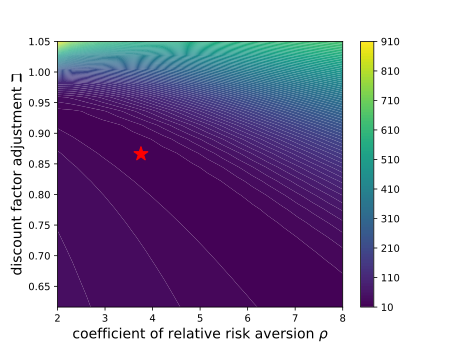
\includegraphics{slides_files/mediabag/../Figures/IndShockSMMcontour.pdf}

\subsection{WUFIM Results}\label{wufim-results}

Model \textbar{} \(\beth\) \textbar{} \(\CRRA\) \textbar{}

\textbar\textbar-\textbar-\textbar{} \textbar{} LCIM w/ Portfolio Choice
\textbar{} 0.866 \textbar{} 3.756 \textbar{} \textbar{} \textbar{}
(0.0011) \textbar{} (0.0313) \textbar{} \textbar{} Separable WUFIM
\textbar{} 0.876 \textbar{} 3.506 \textbar{} \textbar{} \textbar{}
(0.0012) \textbar{} (0.0254) \textbar{} \textbar{} Separable WUFIM w/
Portfolio \textbar{} 0.864 \textbar{} 3.806 \textbar{} \textbar{}
\textbar{} (0.0012) \textbar{} (0.0263) \textbar{} \textbar{}
Non-Separable WUFIM \textbar{} 0.601 \textbar{} 5.032 \textbar{}
\textbar{} \textbar{} (0.0026) \textbar{} (0.0634) \textbar{}

class:center

\subsection{WUFIM Contour Plots}\label{wufim-contour-plots}

class:center

\subsection{Sensitivity Analysis:
Baseline}\label{sensitivity-analysis-baseline}

From Andrews et al.~{[}2017{]}, using finite-difference Jacobians

\includegraphics{slides_files/mediabag/../Figures/IndShockSensitivity.pdf}

class:center

\subsection{Sensitivity Analysis:
Alternatives}\label{sensitivity-analysis-alternatives}

\subsection{Conclusion and Future
Work}\label{conclusion-and-future-work}

\paragraph{Conclusion}\label{conclusion}

\begin{itemize}
\tightlist
\item
  Need wealth in the utility function to better capture distribution of
  wealth
\item
  Need life cycle structure to understand effect of policies on:

  \begin{itemize}
  \tightlist
  \item
    young parents with children and low income
  \item
    working middle aged
  \item
    retirees with low wealth
  \end{itemize}
\end{itemize}

\paragraph{Future Work}\label{future-work}

\begin{itemize}
\tightlist
\item
  Better estimation techniques such as Sequence Space Jacobians (Auclert
  et al.~{[}2021{]})

  \begin{itemize}
  \tightlist
  \item
    Will also help speed up sensitivity analysis
  \end{itemize}
\item
  Implement policy experiments and derive impulse response functions by
  life cycle
\item
  Analyze the effect of policy experiments on different segments of the
  population
\item
  Evaluate optimal policy to minimize differential harm
\end{itemize}



\end{document}
